\documentclass{article}
\usepackage{tikz}
\usetikzlibrary{positioning}

\begin{document}

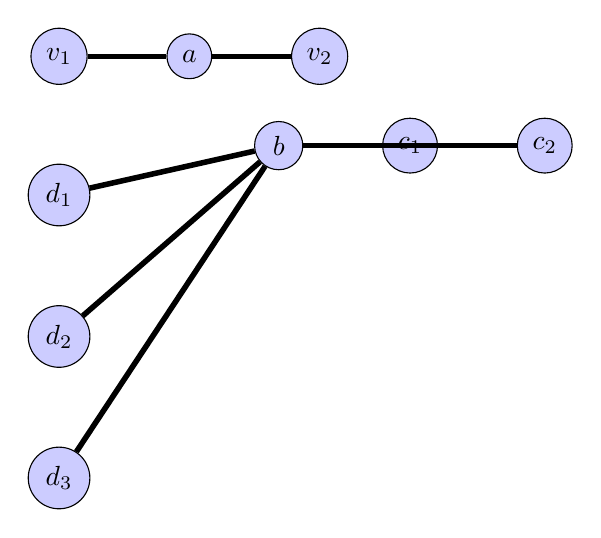
\begin{tikzpicture}[node distance=1cm, every node/.style={circle, fill=blue!20, draw}]
    % Define nodes
    \node (v1) {$v_1$};
    \node[right=of v1] (a) {$a$};
    \node[right=of a] (v2) {$v_2$};
    
    \node[below=of v1] (d1) {$d_1$};
    \node[below=of d1] (d2) {$d_2$};
    \node[below=of d2] (d3) {$d_3$};
    
    \node[below right=of a] (b) {$b$};
    \node[right=of b] (c1) {$c_1$};
    \node[right=of c1] (c2) {$c_2$};
    
    % Draw edges
    \draw (v1) -- (a);
    \draw (a) -- (v2);
    
    \draw (d1) -- (b);
    \draw (d2) -- (b);
    \draw (d3) -- (b);
    
    \draw (b) -- (c1);
    \draw (b) -- (c2);
    
    % Highlight the edges representing G^{(2)}_f
    \draw[line width=2pt] (v1) -- (a);
    \draw[line width=2pt] (a) -- (v2);
    \draw[line width=2pt] (d1) -- (b);
    \draw[line width=2pt] (d2) -- (b);
    \draw[line width=2pt] (d3) -- (b);
    \draw[line width=2pt] (b) -- (c1);
    \draw[line width=2pt] (b) -- (c2);
\end{tikzpicture}

\caption{The neighborhood of \(a \times b\) in \(\mathcal{G}\). The graph \(G^{(2)}_f\) is represented by the pink lines.}
\end{document}